\documentclass[11pt]{amsart}
%prepared in AMSLaTeX, under LaTeX2e
\addtolength{\oddsidemargin}{-.85in}
\addtolength{\evensidemargin}{-.85in}
\addtolength{\topmargin}{-0.85in}
\addtolength{\textwidth}{1.5in}
\addtolength{\textheight}{1.6in}
\newcommand{\normalspacing}{\renewcommand{\baselinestretch}{1.05}
        \tiny\normalsize}

\newtheorem*{thm}{Theorem}
\newtheorem*{defn}{Definition}
\newtheorem*{example}{Example}
\newtheorem*{problem}{Problem}
\newtheorem*{remark}{Remark}

\usepackage{amssymb,fancyvrb,xspace,bm}
\usepackage{palatino}

\usepackage[final]{graphicx}

\usepackage{tikz}
\usetikzlibrary{arrows.meta}

\usepackage{pgfplots}

\usepackage[pdftex, colorlinks=true, plainpages=false, linkcolor=black, citecolor=blue, urlcolor=blue]{hyperref}

% macros
\newcommand{\ba}{\mathbf{a}}
\newcommand{\bb}{\mathbf{b}}
\newcommand{\bbf}{\mathbf{f}}
\newcommand{\bn}{\mathbf{n}}
\newcommand{\br}{\mathbf{r}}
\newcommand{\bu}{\mathbf{u}}
\newcommand{\bv}{\mathbf{v}}
\newcommand{\bx}{\mathbf{x}}
\newcommand{\by}{\mathbf{y}}

\newcommand{\bT}{\mathbf{T}}

\newcommand{\CC}{\mathbb{C}}
\newcommand{\Div}{\nabla\cdot}
\newcommand{\eps}{\epsilon}
\newcommand{\grad}{\nabla}
\newcommand{\ZZ}{\mathbb{Z}}
\newcommand{\ip}[2]{\ensuremath{\left<#1,#2\right>}}
\newcommand{\lam}{\lambda}
\newcommand{\lap}{\triangle}
\newcommand{\RR}{\mathbb{R}}

\newcommand{\prob}[1]{\bigskip\noindent\large\textbf{#1}.\,\normalsize }
\newcommand{\ppart}[1]{\textbf{(#1)}\,\, }
\newcommand{\epart}[1]{\medskip\noindent\textbf{(#1)}\,\, }

\newcommand{\pts}[1]{\scriptsize [#1 points] \normalsize}

\newcommand{\Matlab}{\textsc{Matlab}\xspace}
\newcommand{\Octave}{\textsc{Octave}\xspace}
\newcommand{\Python}{\textsc{Python}\xspace}


\begin{document}
\scriptsize% \phantom{bob} \vspace{-0.3in}
\noindent Math 615 NADE \, (Bueler) \hfill  \today
\normalsize\bigskip
\normalspacing

\Large\centerline{\textbf{2D advection show-and-tell with \textbf{PETSc}}}
\normalsize

\bigskip
\thispagestyle{empty}
\normalspacing

\renewcommand{\labelenumi}{\arabic{enumi}.\,}


\bigskip
\noindent I wrote a book called \emph{PETSc for Partial Differential Equations} which was published by SIAM Press in 2021.  The C and Python example codes from the book are at

\centerline{\href{https://github.com/bueler/p4pdes}{\texttt{github.com/bueler/p4pdes}}}

\noindent Here I will demonstrate a C example which solves a 2D advection problem.  To do this yourself, download and install PETSc (\href{https://petsc.org/}{\texttt{petsc.org}}) and clone the above repository.

\medskip
\noindent \textbf{What is PETSc?}  The \href{https://petsc.org/}{\underline{P}ortable, \underline{E}xtensible \underline{T}oolkit for \underline{S}cientific \underline{c}omputing} is an open and free C numerical software library from Argonne National Laboratory.  It contains iterative linear algebra, nonlinear solvers, mesh management and mesh-aware solvers, and ODE solvers, all implemented in parallel.  It is targeted at high-resolution PDE and multiphysics simulations.  Started before 1995, PETSc co-evolved with the \href{https://www.mpich.org/}{Message Passing Interface} (MPI) as fundamental infrastructure for doing simulations on supercomputers.  The Python finite element library \href{https://www.firedrakeproject.org/}{Firedrake} and the \href{https://www.pism.io/}{Parallel Ice Sheet Model} are two out of \href{https://petsc.org/release/#toolkits-libraries-that-use-petsc}{many examples of scientific computing libraries and applications} which are built on top of PETSc.

Documentation and download for PETSc is at \,\href{https://petsc.org/}{\texttt{petsc.org}}, but it can be installed using a package manager or by installing a higher-level library (e.g.~Firedrake).

\bigskip
\noindent \textbf{Example.}  The C code \,\texttt{advect.c} from Chapter 11 takes a finite difference/volume approach for solving a scalar advection equation in 2D, on $(x,y) \in (-1,1)^2$, with periodic boundary conditions, for $t>0$:
    $$u_t + \nabla \cdot (\mathbf{a} u) = 0$$
The velocity field in this example is a rotational vector field around the origin: $\mathbf{a}(x,y) = \left<y, -x\right>$.  We use an equally-spaced periodic mesh (grid) in $x$ and $y$ to generate the MOL ODE system.  The spatial derivatives, which are needed to compute the flux on the edge of each finite volume cell (dashed in left figure), are approximated with finite differences and a nonlinear, flux-limited, and higher-order upwind scheme; see the figure.  The time-stepping is by a 3rd-order adaptive Runge-Kutta method, suitable for such hyperbolic problems if the fluxes are discretized appropriately.

Here is a parallel example run with visualization, over 4 cores, on a $160\times 160$ spatial grid:

\medskip
\begin{Verbatim}[fontsize=\small]
$ cd c/ch11/ && make advect
$ mpiexec -n 4 ./advect -da_refine 5 -adv_problem rotation \
    -ts_max_time 6.283185 -ts_monitor -ts_monitor_solution draw
\end{Verbatim}

\medskip
A surface plot of the initial condition $u(x,y,0)$ looks like a cone and a square tower (center figure).  The time-dependent solution rotates the initial picture back to the same configuration at $t_f = 2\pi$, but numerical diffusion causes some smoothing of the sharp edges (right figure).  Note the apparent absence of ``ringing'' which we would have gotten from Lax-Wendroff or leap-frog.

\bigskip\medskip
\noindent\mbox{% figure shows large stencil for flux-limiter, and upwind vs far "decision"
\begin{tikzpicture}[scale=1.0]
  \foreach \x in {-2.0,-1.0,0.0,1.0,2.0} {
      \draw[gray,thin] (\x,-2.1) -- (\x,2.1);
  }
  \foreach \y in {-2.0,-1.0,0.0,1.0,2.0} {
      \draw[gray,thin] (-2.1,\y) -- (2.1,\y);
      \filldraw (0.0,\y) circle (1.5pt);
  }
  \foreach \x in {-2.0,-1.0,0.0,1.0,2.0} {
      \filldraw (\x,0.0) circle (1.5pt);
  }
  \draw[dashed] (-0.5,-0.5) -- (0.5,-0.5) -- (0.5,0.5) -- (-0.5,0.5) -- cycle;
  \draw (0.5,0.0) circle (1.5pt);
  \draw (0.0,0.5) circle (1.5pt);
  \draw (-0.5,0.0) circle (1.5pt);
  \draw (0.0,-0.5) circle (1.5pt);
  %\node at (0.25,-0.25) {$V_{ij}$};
  % velocity direction entering cell
  %%\draw[-{Latex[length=2mm]}] (-1.6,0.7) -- (-0.1,0.05) node [midway,below] {$\mathbf{a}$};
  % E upwind decision:
  %\node at (0.7,-0.2) {$E$};
  \path[-{Latex[length=1.5mm]}] (0.45,0.1) edge [bend right] node [midway,above,yshift=-1mm] {\texttt{up}} (0.02,0.1);
  \path[-{Latex[length=1.5mm]}] (0.55,0.1) edge [bend left] node [midway,above] {\texttt{dn}} (0.92,0.1);
  \path[-{Latex[length=1.5mm]}] (0.45,-0.1) edge [bend left] node [midway,below,xshift=-7mm,yshift=1mm] {\texttt{far}} (-0.98,-0.1);
  % N upwind decision:
  %\node at (0.2,0.7) {$N$};
  \path[-{Latex[length=1.5mm]}] (-0.1,0.55) edge [bend left] node [midway,left,xshift=1mm] {\texttt{up}} (-0.1,0.98);
  \path[-{Latex[length=1.5mm]}] (-0.1,0.45) edge [bend right] node [midway,left,xshift=1mm] {\texttt{dn}} (-0.1,0.02);
  \path[-{Latex[length=1.5mm]}] (0.1,0.55) edge [bend right] node [midway,right] {\texttt{far}} (0.1,1.98);

  % generate padding at bottom
  \node at (0.0,-2.4) {\phantom{foo}};
\end{tikzpicture}
 \qquad 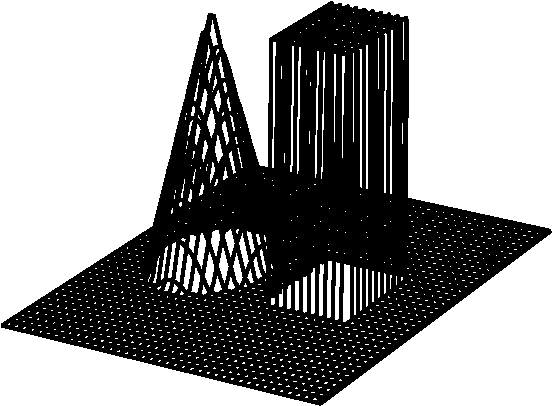
\includegraphics[width=0.34\textwidth]{figs/rotationinitial.pdf} \quad 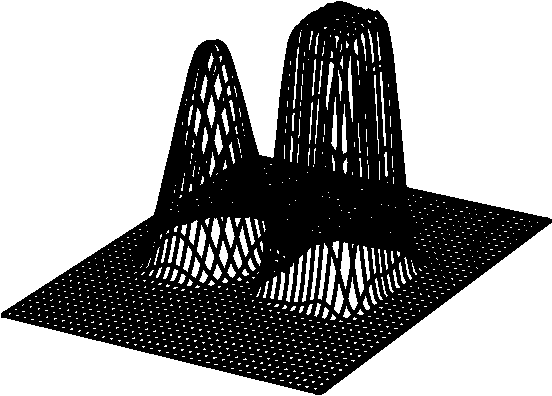
\includegraphics[width=0.34\textwidth]{figs/rotationfinal.pdf}}

\end{document}
